\documentclass[a4paper, 12pt]{article}
\usepackage{graphicx} % Required for inserting images
\usepackage{textcomp}
\usepackage{fullpage}
\usepackage{amsmath}
\usepackage{xcolor}
\usepackage{float}
\usepackage{geometry}
\usepackage{biblatex}
\geometry{margin=1in}
\usepackage{enumitem}
\usepackage{hyperref}
\usepackage{microtype}
\usepackage{gensymb}
\usepackage{parskip}
\usepackage{tikz}
\usepackage{caption}
\usepackage{cancel}
\usepackage{nicefrac}
\hypersetup{
    colorlinks=true,        % Enable colored links
    linkcolor=teal,         % Set color for internal links
    citecolor=teal,         % Set color for citations
    filecolor=teal,         % Set color for file links
    urlcolor=teal           % Set color for URLs
}

\usepackage[version=4]{mhchem}

\newcommand{\degC}{$\degree$C \,}
\newcommand{\degF}{$\degree$F \,}
\newcommand{\R}{\left(0.0821 \: \frac{L \cdot atm}{mol \cdot \text{K}}\right)}
\newcommand{\cunits}{$\frac{J}{g \degree \text{C}}$}
\newcommand{\Hf}{$\Delta H_\text{f}$} % heat of formation
\newcommand{\mathHf}{\Delta H_\text{f}} %heat of formation in math mode

\title{Chemistry Honors Study Guide}
\author{Test 3 S2}
\date{Test date: May 2, 2025}

\begin{document}

\maketitle

\section{Gasses and Heat in Stoichiometry}

\subsection*{Gasses}
$$6 \text{HCl} + 2 \text{Al} \longrightarrow 2 \text{AlCl}_3 + 3\text{H}_2$$

At STP, how many $ml$ of H$_2$ gas are produced from 12 $g$ of solid Al? (1 $mol$ = 22.4 $L$ at STP)

Using stoichiometry:

$$(12 \: g \: \text{Al}) \times \left(\frac{1 \: mol \: \text{Al}}{26.98 \: g \: \text{Al}}\right) \times \left(\frac{3 \: mol \: \text{H}_2}{2 \: mol \: \text{Al}}\right) \times \left(\frac{22.4 \: L \: \text{H}_2}{1 \: mol \: \text{H}_2}\right) \times \left(\frac{1000 \: ml}{1 \: L}\right)$$
$$ = \boxed{14944.4 \: ml}$$

\subsection*{Heats of Formation}
\Hf{} is the heat absorbed/released when compounds are formed from elemental units. The \Hf{} of elements, including diatomic elements, is always 0.

Heats of formation equation:

\begin{equation} \label{heatsofform}
\Delta H_\text{rxn} = \sum \Delta H_\text{f(products)} -  \Delta H_\text{f(reactants)}
\end{equation}

$$\text{CS}_2 + 3\text{O}_2 \longrightarrow \text{CO}_2 + 2\text{SO}_2$$

Find the heat of formation given the following: 

$$\mathHf \: (\text{CO}_2) = -393.5 \: \frac{kJ}{mol}$$
$$\mathHf \: (\text{SO}_2) = -296.8 \: \frac{kJ}{mol}$$
$$\mathHf \: (\text{CS}_2) = 87.9 \: \frac{kJ}{mol}$$

Solution: Using \ref{heatsofform}:

$$ [-393.5 + 2(-296.8)] - [3(0) + 87.9] $$
$$ = \boxed{1075 \: \frac{kJ}{mol}} $$

\section{Redox}

\subsection*{Definitions}

\begin{itemize}[leftmargin=*, nosep]
\item \textbf{\textit{redox reaction}}: Short for \textit{oxidation/reduction reaction}.
\item \textbf{\textit{oxidation}}: Losing electrons (becoming more positive).
\item \textbf{\textit{reduction}}: Gaining electrons (becoming more negative).
\end{itemize}

\subsection*{Reactions}
LEO the lion says GER (Losing Electrons = Oxidation, Gaining Electrons = Reduction)

$$\text{Na} \longrightarrow \text{Na}^+ + e^- \hspace{2em} \text{oxidation \nicefrac12 reaction}$$
$$\text{Cl}_2 + 2e^- \longrightarrow 2\text{Cl}^- \hspace{2em} \text{reduction \nicefrac12 reaction}$$
$$2\text{Na} + \text{Cl}_2 \longrightarrow 2\text{NaCl} \hspace{2em} \text{overall reaction}$$

\subsection*{Assigning Oxidation Numbers}

\subsubsection*{Rules}
\begin{enumerate}
\item An element in its elemental state is neutral.
\item H in a compound is always +1.
\item O in a compound is -2 except for H$_2$O$_2$; in that case, the oxidation number of O is -1.
\item Monatomic ions are whatever ionic charge they would normally form.
\item All oxidation numbers must add to the overall charge of the molecule or ion.
\end{enumerate}

Example: What is the oxidation number of I in Mg(IO$_3$)$_2$?

Solution: By looking at the charge on Mg, the charge on (IO$_3$)$_2$ can be found to be 2-, so the charge on one ion is 1-, making the ion (IO$_3$)$^-$. The oxidation number of O in this compound is 2- by rule 3. There are 3 oxygen atoms, so:

$$3(-2) + \text{I} = -1$$

Solving for I:

$$-6 + \text{I} = -1$$
$$\text{I} = -1+6$$
$$\text{I} = 5$$

The charge on I is \fbox{+5}.

\subsection*{Writing Half-Reactions}
$$2\text{Ag} + \text{H}_2\text{S} \longrightarrow \text{Ag}_2\text{S} + \text{H}_2$$

To write half-reactions, look at the oxidation numbers on each element. If the oxidation number has increased, it has been oxidised. If the number has decreased, it has been reduced.

Oxidation \nicefrac12 reaction:
$$2\text{Ag} \longrightarrow  \text{(break the ionic bond)} \: 2\text{Ag}^+ + 2e^-$$

Reduction \nicefrac12 reaction:
$$2\text{H}^+ + 2e^- \longrightarrow \text{H}_2$$

If \textit{none} of the oxidation numbers change, the reaction is \textit{not} a redox reaction. For example,

$$\text{Al}_2\text{S}_3 + 6 \text{H}_2\text{O} \longrightarrow 2\text{Al(OH)}_3 + 3\text{H}_2\text{S}$$

is not a redox reaction.

\subsection*{Balancing Redox Reactions}
Assume an acidic, aqueous environment:

$$\text{PbO}_2 + \text{I}_2 \longrightarrow \text{Pb}^{2+} + \text{IO}_3^-$$

\begin{enumerate}[leftmargin=*]
\item Separate into oxidation and reduction half-reactions by looking at oxidation numbers.

\begin{gather*}
\text{Oxidation half-reaction:} \: \text{I}_2 \longrightarrow \text{IO}_3^- \\
\text{Reduction half-reaction:} \: \text{PbO}_2 \longrightarrow \text{Pb}^{2+}
\end{gather*}

\item Balance elements that are \textit{not} H or O.

\begin{gather*}
\text{I}_2 \longrightarrow 2\text{IO}_3^- \\
\text{PbO}_2 \longrightarrow \text{Pb}^{2+}
\end{gather*}

\item Balance O by adding H$_2$O.

\begin{gather*}
6\text{H$_2$O} + \text{I}_2 \longrightarrow 2\text{IO}_3^- \\
\text{PbO}_2 \longrightarrow \text{Pb}^{2+} + 2\text{H$_2$O}
\end{gather*}

\item Balance H by adding H$^+$.

\begin{gather*}
6\text{H$_2$O} + \text{I}_2 \longrightarrow 2\text{IO}_3^- + 12\text{H}^+\\
4\text{H}^+ + \text{PbO}_2 \longrightarrow \text{Pb}^{2+} + 2\text{H$_2$O}
\end{gather*}

\item Add electrons to balance the charges. When balanced correctly, electrons should be on opposite sides (one on reactants, one on products). 

\begin{gather*}
6\text{H$_2$O} + \text{I}_2 \longrightarrow 2\text{IO}_3^- + 12\text{H}^+ + 10e^-\\
2e^- + 4\text{H}^+ + \text{PbO}_2 \longrightarrow \text{Pb}^{2+} + 2\text{H$_2$O}
\end{gather*}

\item Multiply to cancel out the electrons.

\begin{gather*}
6\text{H$_2$O} + \text{I}_2 \longrightarrow 2\text{IO}_3^- + 12\text{H}^+ + 10e^-\\
10e^- + 20\text{H}^+ + 5\text{PbO}_2 \longrightarrow 5\text{Pb}^{2+} + 10\text{H$_2$O}
\end{gather*}

\item Combine and cancel.

\begin{gather*}
\cancel{6\text{H$_2$O}} + \text{I}_2 \longrightarrow 2\text{IO}_3^- + \cancel{12\text{H}^+} + \cancel{10e^-}\\
\cancel{10e^-} + \cancel{20\text{H}^+} 8\text{H}^+ + 5\text{PbO}_2 \longrightarrow 5\text{Pb}^{2+} + \cancel{10\text{H$_2$O}} 4\text{H$_2$O} \\
\boxed{\text{I}_2 + 8\text{H}^+ + 5\text{PbO}_2 \longrightarrow 5\text{Pb}^{2+} + 4\text{H$_2$O} + 2\text{IO}_3^-}
\end{gather*}

\end{enumerate}

\section{Batteries}
Below is a diagram of a Voltaic/Galvanic cell:
\begin{figure}[H]
\centering
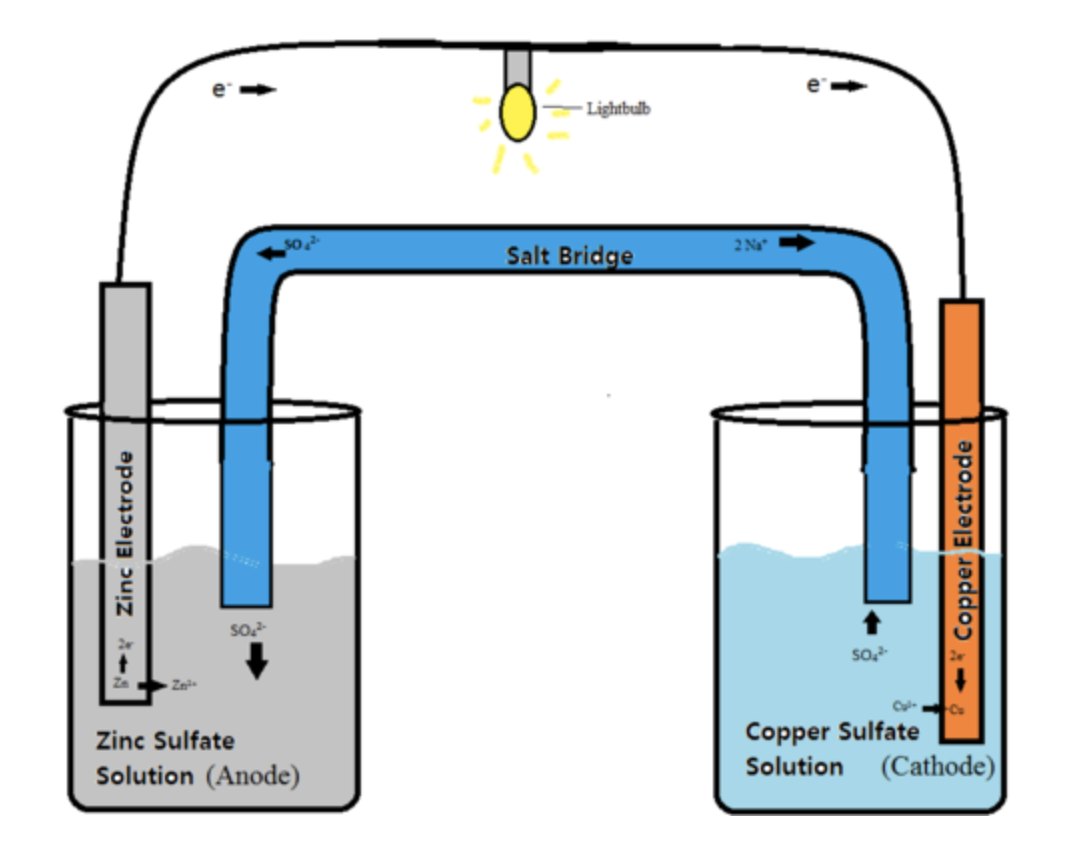
\includegraphics[width=0.6\textwidth]{voltaiccell}
\end{figure}

containing:

\begin{description}
\item[electrodes] to carry electricity. The \textbf{anode} is oxidised, losing mass as the material is released into solution, and the \textbf{cathode} is reduced, gaining mass as solid metal deposits onto it.
\item[salt bridge] to close the circuit. 
\item[solutions] that the electrodes are suspended in. 
\end{description}

Electrons flow from the anode to the cathode.

To find the voltage of this battery:

$$\text{Cu}^{2+} + 2e^- \longrightarrow \text{Cu} \: (0.34 \: \text{V})$$
$$\text{Zn}^{2+} + 2e^- \longrightarrow \text{Zn} \: (-0.726 \: \text{V})$$

Flip the equation that is higher on the standard reduction potential table:

$$\text{Cu}^{2+} + 2e^- \longrightarrow \text{Cu} \: (0.34 \: \text{V})$$
$$\text{Zn} \longrightarrow \text{Zn}^{2+} + 2e^- \: (0.726 \: \text{V})$$

Combine:

$$\text{Cu}^{2+} + \text{Zn} \longrightarrow \text{Cu} + \text{Zn}^{2+} \: \boxed{(1.1 \: \text{V})}$$

\textsc{n.b.} When \textbf{multiplying} an equation to balance out the electrons, \textbf{the voltage does not change.} It only changes in sign if the equation is flipped.

\end{document}